On considère le cube $ABCDEFGH$ de côté 1, le milieu $I$ de $[EF]$ et $J$ le symétrique de $E$ par rapport à $F$.

\begin{center}
	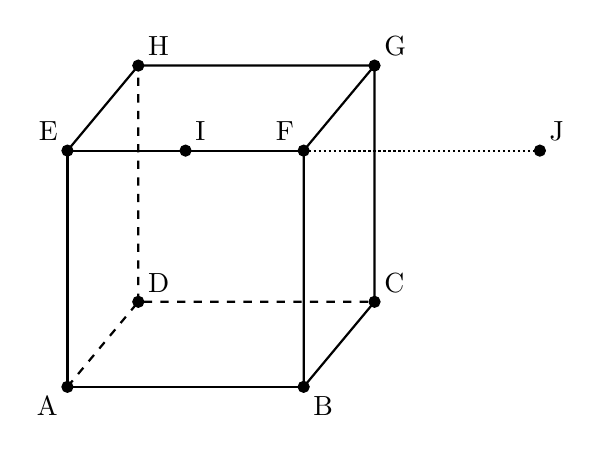
\begin{tikzpicture}[x=0.6cm,y=0.6cm]
		\draw[thick] (0,0)--(5,0)--(5,5)--(0,5)--cycle ;
		\draw[thick] (5,0)--(6.5,1.8)--(6.5,6.8)--(5,5)--cycle;
		\draw[thick] (0,5)--(1.5,6.8)--(6.5,6.8);
		\draw[thick,dashed] (0,0)--(1.5,1.8)--(6.5,1.8) (1.5,1.8)--(1.5,6.8);
		\draw[thick,densely dotted] (5,5)--(10,5) ;
		\foreach \Point/\Name/\Pos in {(0,0)/A/below left,(5,0)/B/below right,(6.5,1.8)/C/above right,(1.5,1.8)/D/above right,(0,5)/E/above left,(5,5)/F/above left,(6.5,6.8)/G/above right,(1.5,6.8)/H/above right,(2.5,5)/I/above right,(10,5)/J/above right}
		\filldraw \Point circle(2pt) node[\Pos] {\Name} ;
	\end{tikzpicture}
\end{center} 

Dans tout l'exercice, l'espace est rapporté au repère orthonormé $\left( A;\vect{AB},\,\vect{AD},\,\vect{AE} \right)$.

\begin{enumerate}
	\item
	\begin{enumerate}
		\item Par lecture graphique, donner les coordonnées des points $I$ et $J$.
		\item En déduire les coordonnées des vecteurs $\vect{DJ}$, $\vect{BI}$ et $\vect{BG}$.
		\item Montrer que $\vect{DJ}$ est un vecteur normal au plan $(BGI)$.
		\item Montrer qu’une équation cartésienne du plan $(BGI)$ est : $2x-y+z-2=0$.
	\end{enumerate}
	\item On note $d$ la droite passant par $F$ et orthogonale au plan $(BGI)$.
	\begin{enumerate}
		\item Déterminer une représentation paramétrique de la droite $d$.
		\item On considère le point $L$ de coordonnées $\left(\dfrac23;\dfrac16;\dfrac56\right)$.
		
		Montrer que le point $L$ est le point d'intersection de la droite $d$ et du plan $(BGI)$.
	\end{enumerate}
	\item On rappelle que le volume $\mathcal{V}$ d'une pyramide est donné par la formule \[ \mathcal{V}=\dfrac13 \times \mathcal{B} \times h \] où $\mathcal{B}$ est l'aire d'une base et $h$ la hauteur associée à cette base.
	\begin{enumerate}
		\item Calculer le volume de la pyramide $FBGI$.
		\item En déduire l'aire du triangle $BGI$.
	\end{enumerate}
\end{enumerate}

